\usepackage[authoryear,round]{natbib}
\usepackage{multirow}

\newcommand{\sheetnum}{%
	04
}
%\setcounter{section}{\sheetnum-3}
\newcommand{\tutorialtitle}{%
    Density Transformation
}
\newcommand{\tutorialtitleshort}{%
    Density Transformation
}
% for slides
\subtitle{\sheetnum \tutorialtitle}

%\maxdeadcycles=1000 % Workaround for ! Output loop---100 consecutive dead cycles because of too many figures

% The following use of algroithms does not work well with the notes:
%
%
%
%
% instead use the following for your algorithms:
%
%\begin{figure}[!t]
%\removelatexerror
%\begin{algorithm}[H]
    % your algo here
    %\label{alg:algolabel}
    %\caption{algocaption}
%\end{algorithm}
%\end{figure}
%\begin{algorithm}
% Below is the definition for the command \removelatexerror:
\makeatletter
\newcommand{\removelatexerror}{\let\@latex@error\@gobble}
\makeatother

\begin{document} %%%%%%%%%%%%%%%%%%%%%%%%%%%%%%%%%%%%%%%%%%%%%%%%%%%%%%%

\sheet{\sheetnum}{\tutorialtitleshort}

\ttopic{\tutorialtitle}

\columnratio{0.2,0.8}\textbf{}
\begin{paracol}{2}
%\setlength{\columnseprule}{0.1pt}
%\setlength{\columnsep}{5em}

\begin{rightcolumn}

% notes version will ignore it
\begin{frame}
\titlepage
\end{frame}

\begin{frame}
\tableofcontents
\end{frame}

\newpage

\mode<all>

\section{The ICA problem:}

Let $\vec s = (s_1, s_2,...,s_N)^\top$ denote the concatenation of independent sources 
and $\vec x \in \R^N$ describe our observations. $\vec x$ relates to $\vec s$ through a 
\emph{linear transformation} $\vec A$:

\begin{equation}
\label{eq:ica}
\vec x = \vec A \, \vec s.
\end{equation}

We refer to $\vec A$ as the \emph{mixing matrix} and Eq.\ref{eq:ica} as the \emph{ICA problem}, 
which is recovering $\vec s$ from only observing $\vec x$.

\underline{Example scenario:}

Two speakers are placed in a room and emit signals $s_1$ and $s_2$. 
The speakers operate indepdendent of one another.  
Two microphones are placed in the room and start recording. 
The first microphone is placed slightly closer to speaker 2, while 
the second microphone is placed slightly closer to speaker 1.
$x_1$ and $x_2$ denote the recordings of the first and second microphone respectively. 
When we listen to the recordings we expect to hear a mix of $s_1$ and $s_2$. 
Since microphone 1 was placed closer to speaker 2, when we only listen to $x_1$ we hear more of $s_2$ than $s_1$. 
The opposite can be said when we listen only to $x_2$.

Acoustic systems are linear. This means that $x_1$ is a superposition of \emph{both} sources $s_1$ and $s_2$. 
We will assume here that the contribution of a source $s_i$ 
to an observation $x_j$ is inversely proportional to the distance between the source and the microphone. 
The distance-contribution relationship is \emph{linear}. We don't need this to be any more realistic. 

If we had a measurement of the distance between each microphone and each speaker, 
we would tell exactly what the contribution of each of $s_1$ and $s_2$ is to each recorded observation. 
If we know the exact contribution of a source to an observation, we can look at both observations and recover each source in full.

This is what ICA tries to solve, except that it does not have any knowledge about the spatial setting. It is blind.

\underline{Outline:}

Before we tackle ICA itself, we first look at the more basic principle of \emph{density transformation} and 
the \emph{convservation of probability}.\\
We start with more specific cases of applying density transformations, 
namely \emph{pseudo random number generators} and what the inverse of \emph{cumulative distribution functions (cdf)} can be used for.\\
Finally we discuss how to generalize this in order to transform one probability density function (pdf) into another.

\subsection{PRNG:}

How can we sample from the uniform distribution $\in \lbrack0, 1)$?

\begin{itemize}
\item Create a sequence, preferrably with a wrong period.
\item minimal pattern and sub-subsequences
\item determinism has an advantage:
\begin{enumerate}
	\item \emph{reproducible} sequneces
	\item efficiency; the starting element or ``seed'' and length of the sequence is suffcient is representative of the entire sequnece.
\end{enumerate}
\end{itemize}

\underline{Linear congruential generator (LCG):}

Start with a seed $y_0 \in \overbrace{\left\{0,\ldots,m-1\right\}}^{=:\;\mathcal{M}}$ with $m \in \N$ ($m$ controls the granularity). 
The next sample $y_t$ is computed as:

\begin{equation}
y_t = \left( \, a \; y_{t-1} \; + \; b \, \right) \, \text{mod} \; m,
\end{equation}
where\\[-0.7cm]
\begin{align*}
a \in \mathcal{M}&\; \text{is the multiplier,} \\
b \in \mathcal{M}&\; \text{is the increment.}
\end{align*}

Then $u_i = \frac{y_i}{m} \approx \,\mathcal{U} \in \lbrack0, 1)$.

Although finicky and requiring careful parameterization, LCG gives us something for drawing from a uniform distribution. 
Next, we look at how to draw samples of a random variable $X$ with a desired pdf $p_X(x)$. 
using uniformly sampled values $\tilde z \in [0,1]$.

\subsection{Inverse CDF:}

If $F_{X}(x)$ is the cumulative
  distribution function (cdf) of a random variable $X$, then the
random variable $Z = F_{X}(X)$ is uniformly distributed on the
interval $[0,1]$. This result provides 
% (after inverting the relationship) 
a general recipe to generate
samples $\tilde x$ of a random variable $X$ with a desired pdf $p_X(x)$
from uniformly distributed random numbers $\tilde z \in [0,1]$:
\begin{enumerate}
\item Compute the cdf $F_X(x)$ of the desired pdf $p_X(x)$

\begin{equation}
F_X(x) = P(X \leq x) = \int_{-\infty}^{x} p(y)\,dy
\end{equation}

The cdf is a one-to-one mapping of the domain of the cdf to the interval $[0,1]$.
 If $Z$ is a uniform random variable, then $X=F_X^{-1}(Z)$ has the distribution $F$.

\item Determine the inverse transformation $F^{-1}$.

\item Sample uniformly distributed numbers (in $[0,1]$), $\tilde z$.
\item Get the samples $\tilde x=F^{-1}(\tilde z)$ from $X$. 
\end{enumerate}

At this point we can use a PRNG to sample from the uniform distribution and 
by plugging those samples into the inverse cdf we can obtain samples from a desired pdf.

\newpage

\section{Density Transformation:}

Let $X_1$ and $X_2$ be jointly continuous random variables with 
density function $f_{X_1, X_2}$:

$$
f_{X_1, X_2}(x_1, x_2) = f(\vec x) \qquad \vec x \in \Omega \subset \R^2
$$

and let $\vec u = \vec u(\vec x) = ( u_1(\vec x), u_2(\vec x)) = ( u_1(x_1, x_2), u_2(x_1, x_2)) $ be a one-to-one mapping/transformation.

%\begin{figure}
%\centering
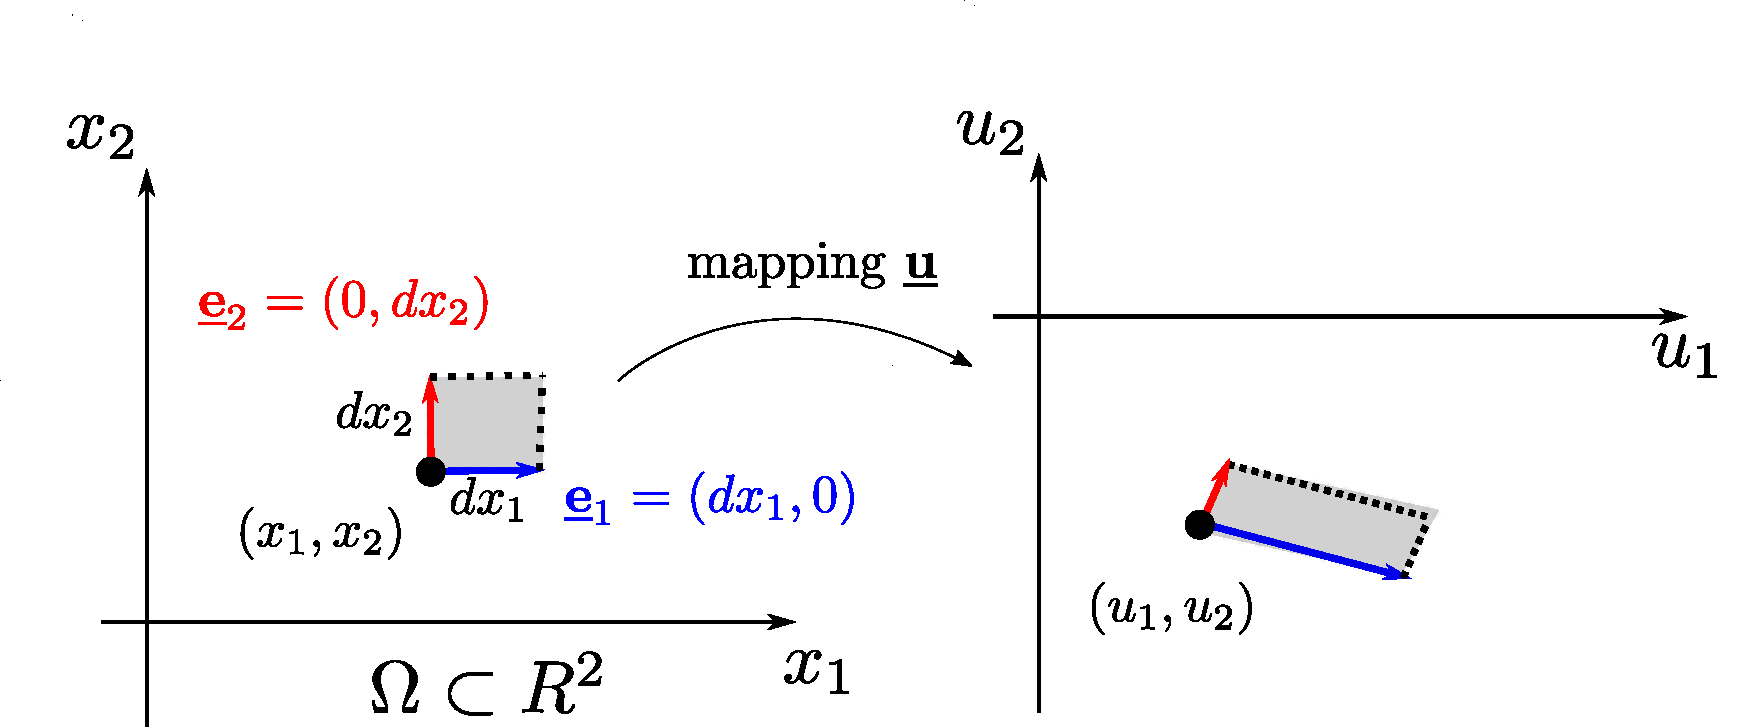
\includegraphics[width=0.7\textwidth]{img/u.pdf}
%\caption*{$\vec{\psi} \in \mathcal{F} = \overline{\operatorname{span} \vec{\phi}(\mathbb{R}^N)}$}
%\end{figure}

The area of the small rectangle in $\Omega$ is $A = dx_1\, dx_2$.\\

The goal is to show that in order for probability to be conserved, the areas on both spaces have to be equal. 
We will therefore demonstrate that:
$$
\int_{\Omega} f(\vec{x}) \mathbf{d}\vec{x}
=\int_{u(\Omega)} f({\vec x(\vec u)}) \frac{1}{\left|\det \frac{\partial \vec{u}(\vec{x})}{\partial \vec{x}} \right|} \mathbf{d}\vec{u}.
$$

\begin{itemize}
\item Because $dx_1$ and $dx_2$ are \emph{infinitesimally small} we can consider the mapping 
$\vec u$ to act as a linear transformation, resulting in a different shape in $u(\Omega)$. 
\item The shape of the shaded area in $u(\Omega)$ is \emph{approximately} a parallelogram.
\item We will compute the ratio of the areas between the two transforms.
\item If we want to go back from $u(\Omega)$ to $\Omega$ we only need $\frac{1}{\text{ratio}}$.
\end{itemize}

\underline{Important:}
Approximating the above as a linear transformation (i.e. a small rectangle turns into a parallelogram) only holds because for very small $d\vec x$.

To get the area of the parallelogram in $u(\Omega)$ we need to find out what $\vec u(dx_1, dx_2))$ is.
The area of the parallelogram then becomes the magnitude of the cross product between the components of $\vec u(\vec x)$.

\newpage

We first only consider the vector due to $dx_1$ in blue:

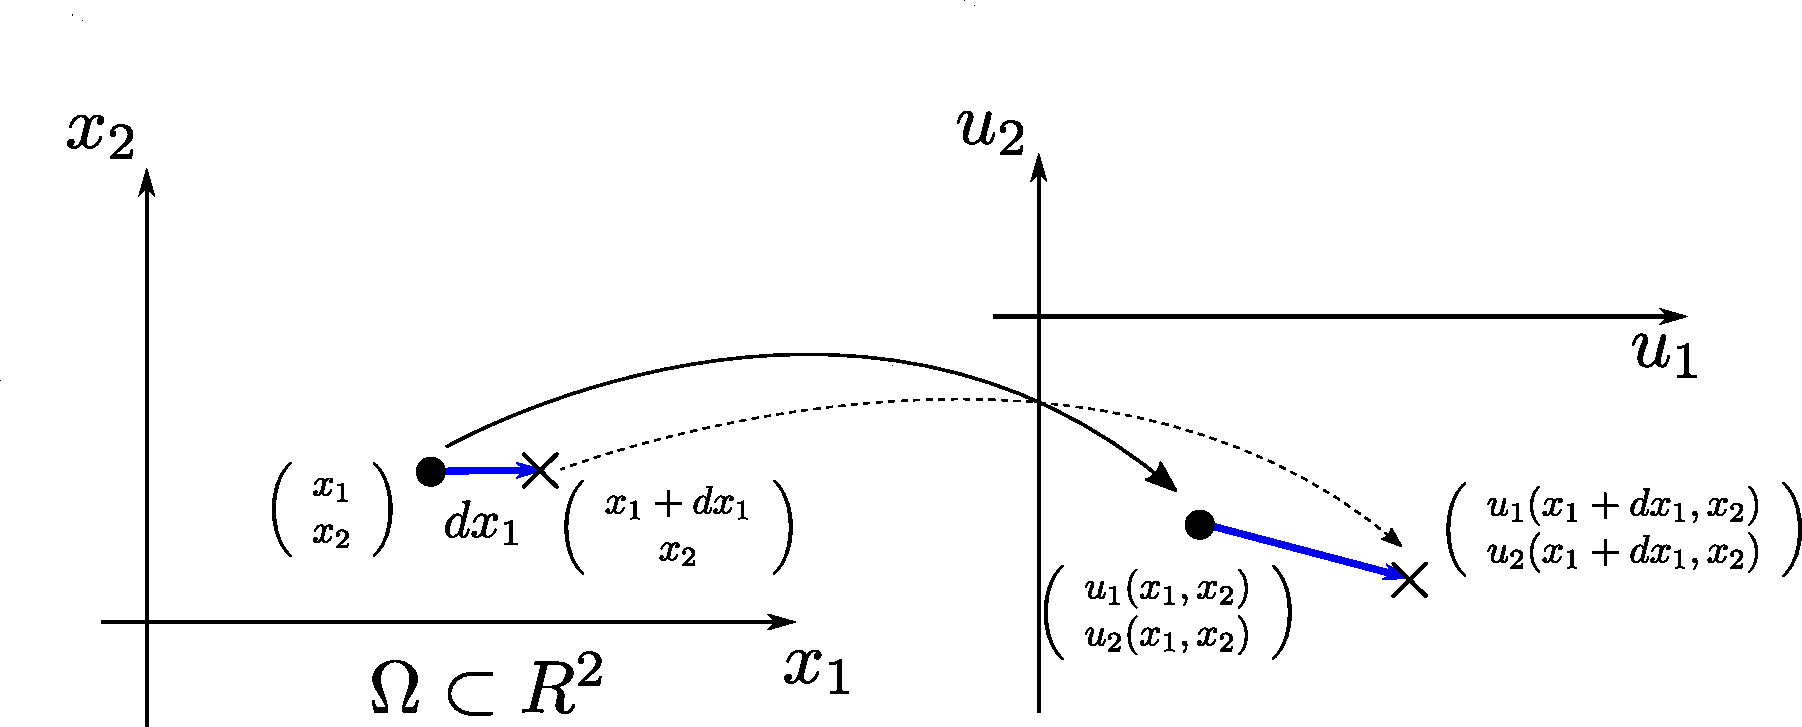
\includegraphics[width=0.75\textwidth]{img/x1.pdf}

The difference vector between the two correspsonding points in $u(\Omega)$ becomes:

\begin{equation*}
\begin{array}{r}
\rmat{
u_1 (x_1 + dx_1, x_2)\\
u_2 (x_1 + dx_2, x_2)
} - 
\rmat{
u_1 (x_1, x_2)\\
u_2 (x_1, x_2)
} \\[0.7cm]
=
\rmat{
u_1 (x_1 + dx_1, x_2) - u_1 (x_1, x_2)\\
u_2 (x_1 + dx_2, x_2) - u_2 (x_1, x_2)
}
\end{array}
\end{equation*}

Because $dx_1$ is so small, we can approximate the transformed vector by the derivative, 
which is essentially taking the limit. The difference vector in $u(\Omega)$ becomes:

$$
u: \vec e_1 \mapsto 
\rmat{
\frac{\partial u_1}{\partial x_1} \Delta x_1\\[0.2cm]
\frac{\partial u_2}{\partial x_1} \Delta x_1
}
$$

\question{What about $dx_2$?}

- We use the same procedure (one the red vector $\vec e_2$) and get:

$$
u: \vec e_2 \mapsto 
\rmat{
\frac{\partial u_1}{\partial x_2} \Delta x_2\\[0.2cm]
\frac{\partial u_2}{\partial x_2} \Delta x_2
}
$$

The area of the parallelogram spanned by the two difference vectors in $u(\Omega)$ 
is the magnitude of their cross product:
\begin{align*}
&\left| \; 
\rmat{
\frac{\partial u_1}{\partial x_1} \Delta x_1\\[0.2cm]
\frac{\partial u_2}{\partial x_1} \Delta x_1
}
\times
\rmat{
\frac{\partial u_1}{\partial x_2} \Delta x_2\\[0.2cm]
\frac{\partial u_2}{\partial x_2} \Delta x_2
}
\; \right|\\ 
&=
\left| \; 
\underbrace{
\frac{\partial u_1}{\partial x_1} \frac{\partial u_2}{\partial x_2}
\; - \;
\frac{\partial u_1}{\partial x_2} \frac{\partial u_2}{\partial x_1}
}_{\text{the Jacobian determinant}}
\; \right| \Delta x_1 \Delta x_2 \\
&= 
\left| \; \det \quad
\underbrace{
\left(
\frac{\partial (u_1, u_2)}{\partial (x_1,x_2)}
\right)
}_{\text{the Jacobian}}
\; \right| \Delta x_1 \Delta x_2
\end{align*}

This matrix of partial derivatives is called the \emph{Jacobian}:
$$
\frac{\partial (u_1, u_2)}{\partial (x_1,x_2)} = 
\frac{\partial (u_1(\vec x), u_2(\vec x))}{\partial (x_1,x_2)} = 
\frac{\partial (\vec u(\vec x))}{\partial (\vec x)} =
\underbrace{
\rmat{
{\partial u_1}/{\partial x_1} & {\partial u_1}/{\partial x_2}\\[0.2cm]
{\partial u_2}/{\partial x_1} & {\partial u_2}/{\partial x_2}
}%rmat
}_{
\substack{
\text{matrix of}\\
\text{partial derivatives}
}%substack
}
$$

If we are given an area spanned by too small vectors (e.g. $\vec e_1$, $\vec e_2$) 
we can compute the area of the corresponding parallelogram in $u(\Omega)$ 
by multiplying the original area by the Jacobian determinant.

\question{What if we want to transform from $u(\Omega)$ back to $\Omega$?}

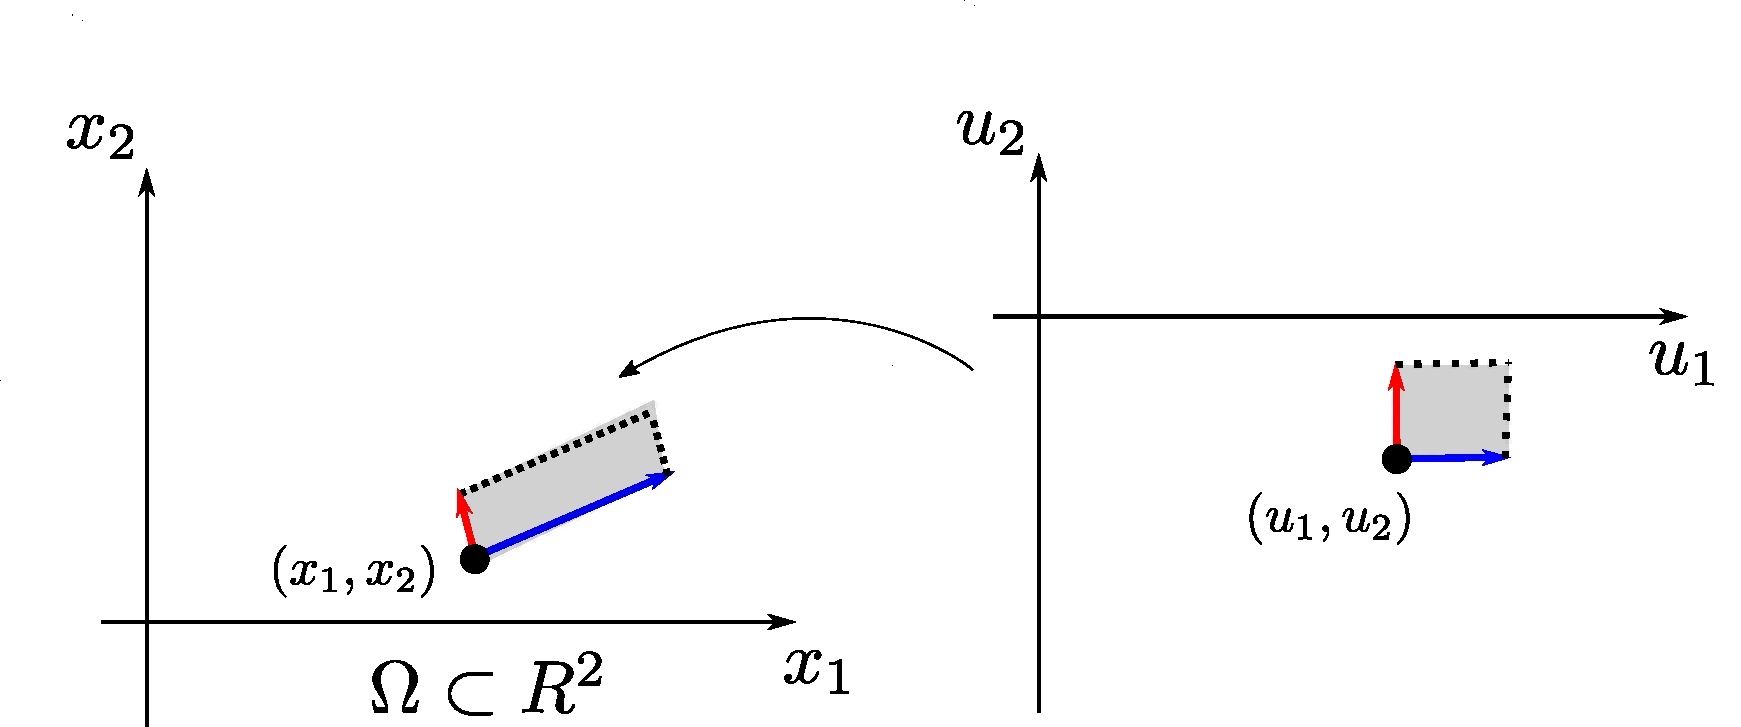
\includegraphics[width=0.7\textwidth]{img/reverse.pdf}

We apply the inverse mapping. A very small rectangle in $u(\Omega)$ transforms into a parallelogram in $\Omega$. 
This reverse transformation would require the inverse of the above matrix of partial derivatives.
The matrix of partial derivatives tells us how to transform infinitesimally small vectors back and forth.

%Transformation between the spaces for infinitesimally small vectors:

%$$
%\rmat{
%u_1(x_1) & u_1(x_2)\\
%u_2(x_1) & u_2(x_2)
%}
%\rmat{
%a\\
%b
%}
%=
%\rmat{
%u_1(x_1)\\
%u_2(x_1)
%}
%a
%+
%\rmat{
%u_1(x_2)\\
%u_2(x_2)
%}
%b
%$$

\question{Do we really have to compute the inverse of the matrix?}

- No, the determinant of the inverse matrix is 1 / det of the original matrix:
$$
\frac{1}{\left| \det \left( \frac{\partial \vec u}{\partial \vec x} \right) \right|} =
{\left| \det \left( \frac{\partial \vec x}{\partial \vec u} \right) \right|}
$$

\underline{Transformation between probability densities:}

Conservation of probability: The area represents the probability of the event, 
transforming it into another space should nt cause any increase or decrease in the probability of the event.

Therefore, if we multiply the area of the rectangle in $\Omega$ by the pdf $f(\vec x)$ at $\vec x$, we get the probability of the parallelogram in $u(\Omega)$:

$$
\int_{\Omega} f(\vec{x}) \mathbf{d}\vec{x}
=\int_{u(\Omega)} f({\vec x(\vec u)}) \left|\det \frac{\partial \vec{x}(\vec{u})}{\partial \vec{u}} \right| \mathbf{d}\vec{u}
$$
$$
=\int_{u(\Omega)} f({\vec x(\vec u)}) \frac{1}{\left|\det \frac{\partial \vec{u}(\vec{x})}{\partial \vec{x}} \right|} \mathbf{d}\vec{u}.
$$


\mode*

\clearpage

%\section{References}
%\begin{frame}[allowframebreaks] \frametitle{References}
	%\scriptsize
	%\bibliographystyle{plainnat}
	%\bibliography{bibliography}
%\end{frame}

\end{rightcolumn}
\end{paracol}

\end{document}
